\documentclass[
	a4paper,
	12pt
]{article}

\PassOptionsToPackage{
	right=2.5cm,
	left=2.5cm,
	top=2.5cm,
	bottom=2.5cm
}{geometry}

\usepackage{
	geometry,
	graphicx,
	parskip
}

\title{[RFC] Linear Algebra Functionality (Issue \#28)}
\author{Fikri Ajiwijaya}
\date{}

\begin{document}

\maketitle

\section{Your Background}

\subsection{Full name}
Fikri Ajiwijaya

\subsection{University status}
Yes

\subsection{University name}
Institut Teknologi Sepuluh Nopember

\subsection{University program}
Mathematics

\subsection{Expected graduation}
April 18th, 2026

\subsection{Short biograph}

I am a recent Pure Mathematics graduate from the Institut Teknologi Sepuluh Nopember, where I specialized in linear algebra and graph theory. My academic background focuses on the intersection of rigorous mathematical theory and computational efficiency, specifically using tools like NumPy and the Z3 Solver for constraints formulations.

Technically, I am a polyglot developer with a long history in C, C++, and OpenGL, where I developed a deep understanding of memory management and real-time graphics pipelines. More recently, I have focused on the JavaScript/Node.js ecosystem, having experience with vanilla JavaScript for the browser and gaining experience with TypeScript and node:test frameworks.

My primary interest lies in high-performance numerical computing. I am motivated to bridge the gap between abstract mathematical routines and web-based execution environments, ensuring that the JavaScript standard library can support the next generation of scientific computing and 3D visualization.

\subsection{Timezone}
UTC+7 (Jakarta)

\subsection{Contact details}
email:fikri.ajiwijaya@gmail.com,
github:fikri-ajiwijaya,
whatsapp:+62816602571

\section{Programming Experience}

\subsection{Platform}
Windows

\subsection{Editor}

I specifically use the stack of VSCode + Docker to program inside of devcontainer.

I use the VSCode Neovim extension + installing Neovim on the host, so that I can use VIM motions in VSCode.

Due to this setup, I have become platform agnostic, having work in all Windows + WSL 2, MacOS, and Linux.

Similarly, I also enable VIM mode in XCode.

\subsection{Programming experience}

\textit{(2025)} \textbf{Metric Dimension}

\textit{using Python, numpy, Z3 Solver}

\begin{center}
	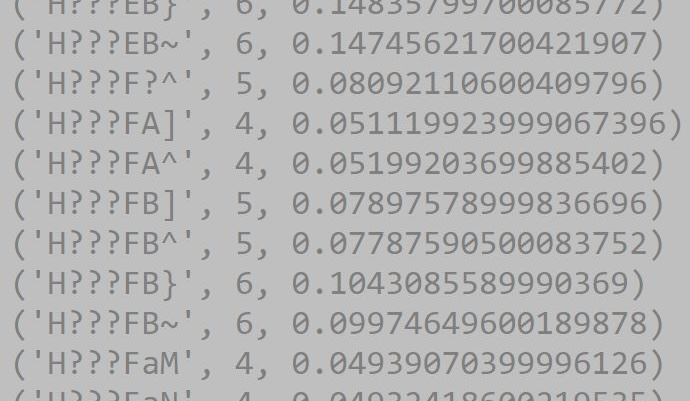
\includegraphics[height=3cm]{img/metric-dimension}
\end{center}

This project was about determining the metric dimension and edge metric dimension of graphs using satisfiability modulo theories. What I did here was to transform the problem using matrix algebra into a new form that I call as reduced distance similarity matrix and reduced edge distance similarity matrix. After which, I based on these matrices, I formulate them into constraints in satisfiability modulo theories.

\pagebreak
\textit{(2024)} \textbf{Cobit Tools}

\textit{using JavaScript}

\begin{center}
	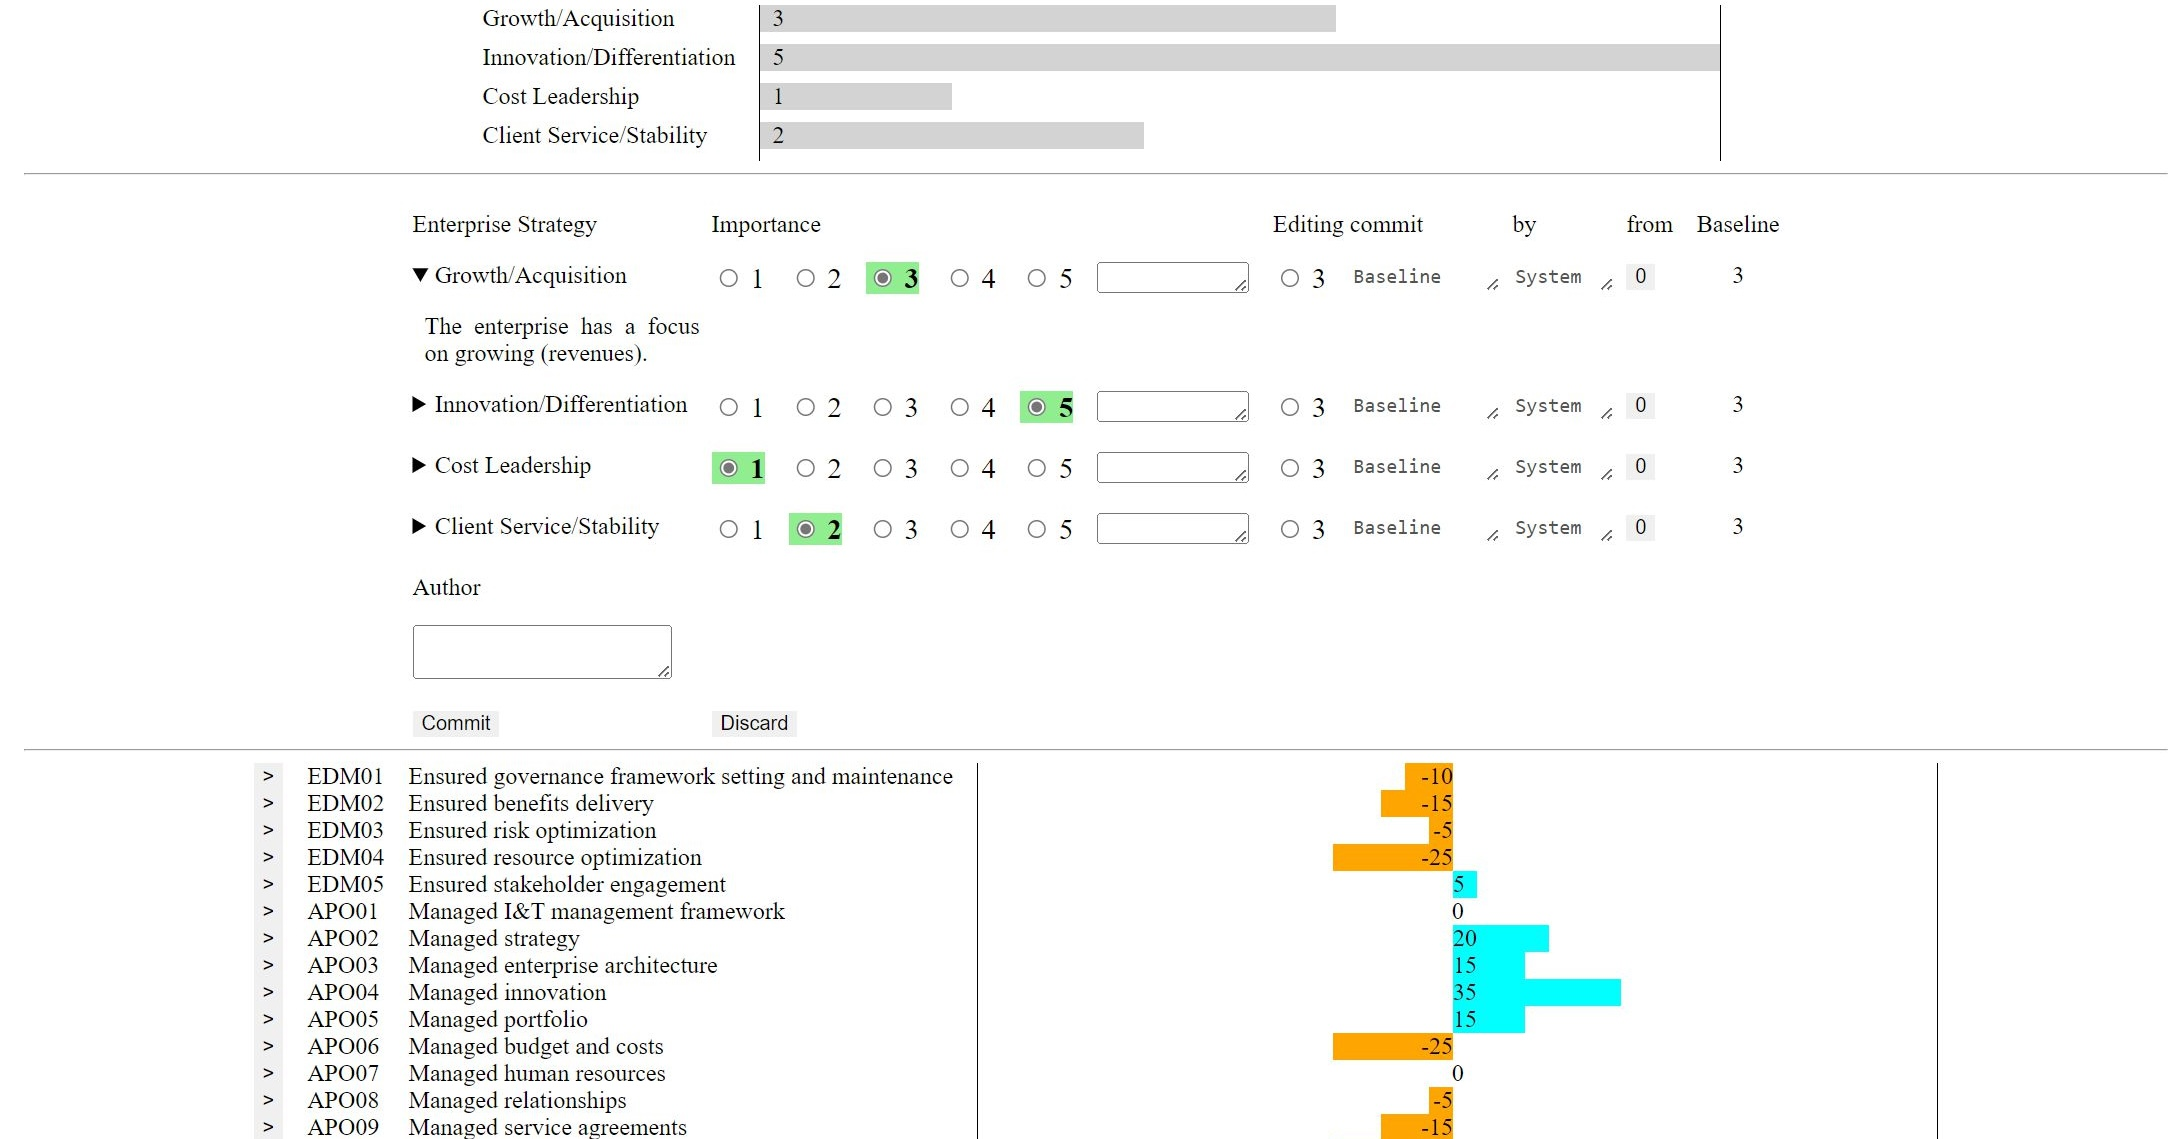
\includegraphics[height=3cm]{img/cobit-tools}
\end{center}

COBIT (Control Objectives for Information and Related Technology) is framework for IT governance and management. This project was about creating a web interface to be able to calculate GMO (Governance Management Objectives) scores based on some design factors input, such as enterprise strategy, risk appetite, compliance requirements, etc. In this project, I hand coded some matrix operations in vanilla JavaScript for the calculations of the GMO scores based on some predetermined weight matrices.

\textit{(2023)} \textbf{Refilter}

\textit{using PHP, PostgreSQL, JavaScript}

\begin{center}
	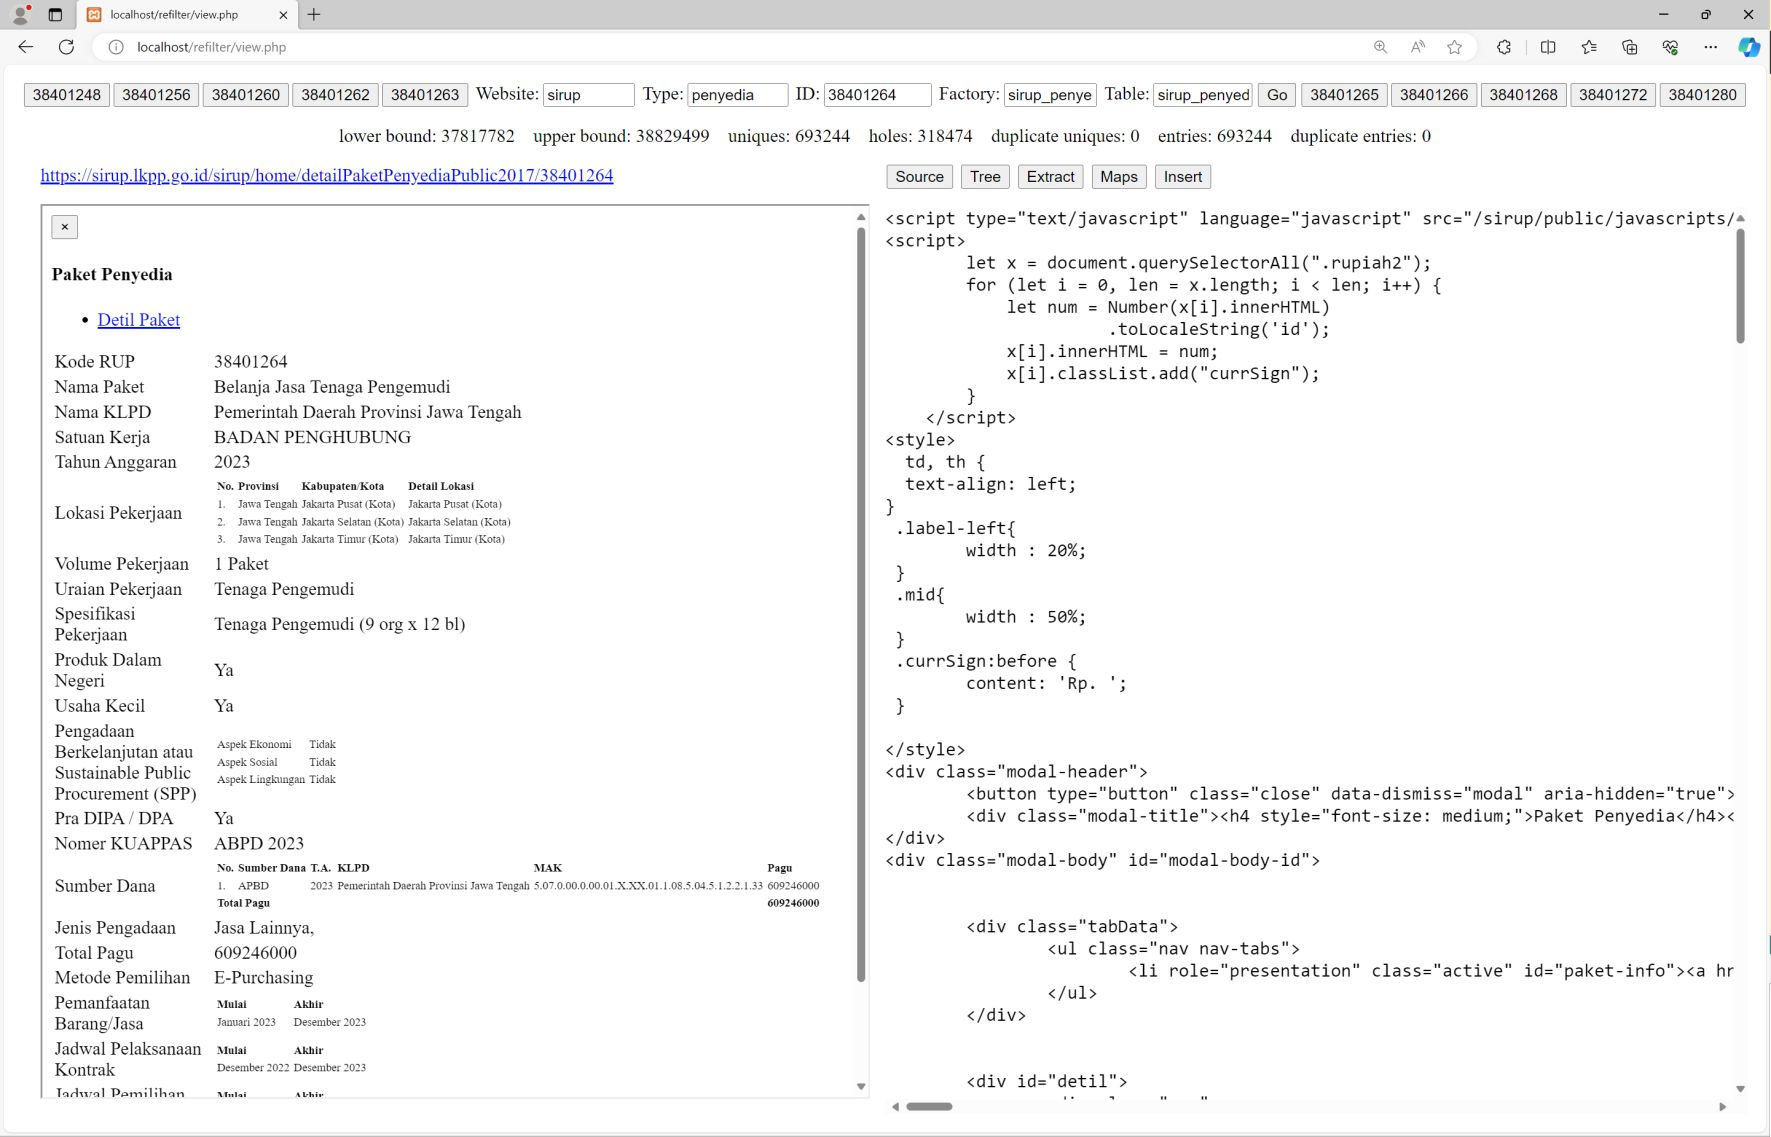
\includegraphics[height=3cm]{img/refilter}
\end{center}

This project was about gathering data for business intelligence from two procurement platforms of Indonesian governent; they are SIRUP LKPP and MODI. Neither platform providing any official API to access their data directly, hence this was a data scraping project. Here, I've learned a lot about parsing DOM documents, understanding their structure, and how to query and select them using XPath.

\textit{(2022)} \textbf{Inkindo Billing}

\textit{using Python, numpy, pandas, DashPlotly}

\begin{center}
	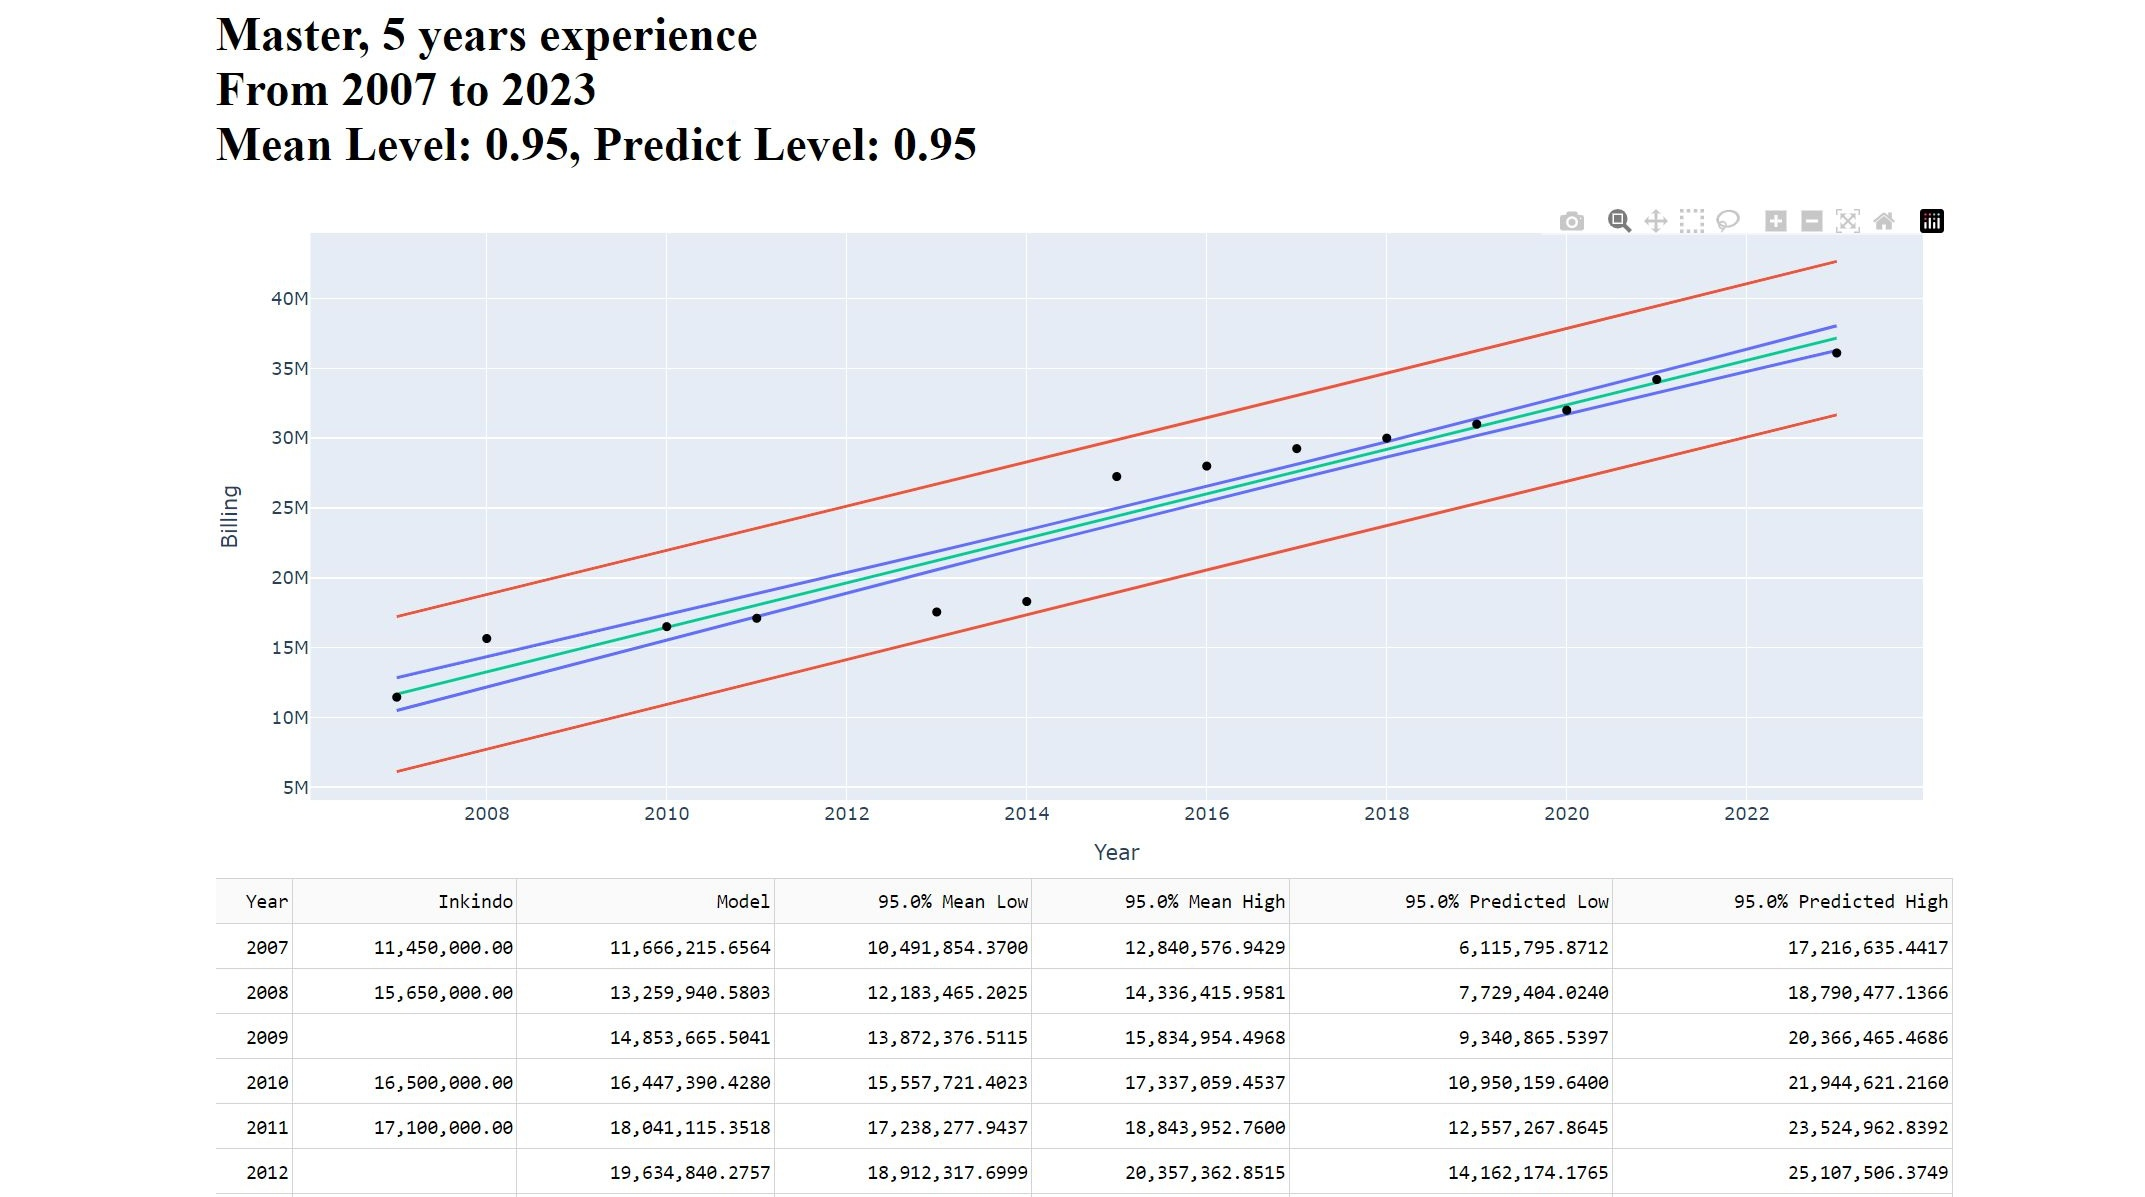
\includegraphics[height=3cm]{img/inkindo-billing}
\end{center}

INKINDO is the national association of Indonesian consultants, an organization for independent consulting firms in Indonesia. This organization releases consultant fee standards annually. However, this billing guidelines often arrive late in the fiscal planning cycle. This project was about analyzing historical INKINDO billing data to build a predictive model that could estimate upcoming figures in advance, enabling better planning and strategic preparation. The statistical method that I used here was multivariable linear regression.

\pagebreak
\textit{(2022)} \textbf{Curriculum Graph}

\textit{using Python, pandas, DashPlotly}

\begin{center}
	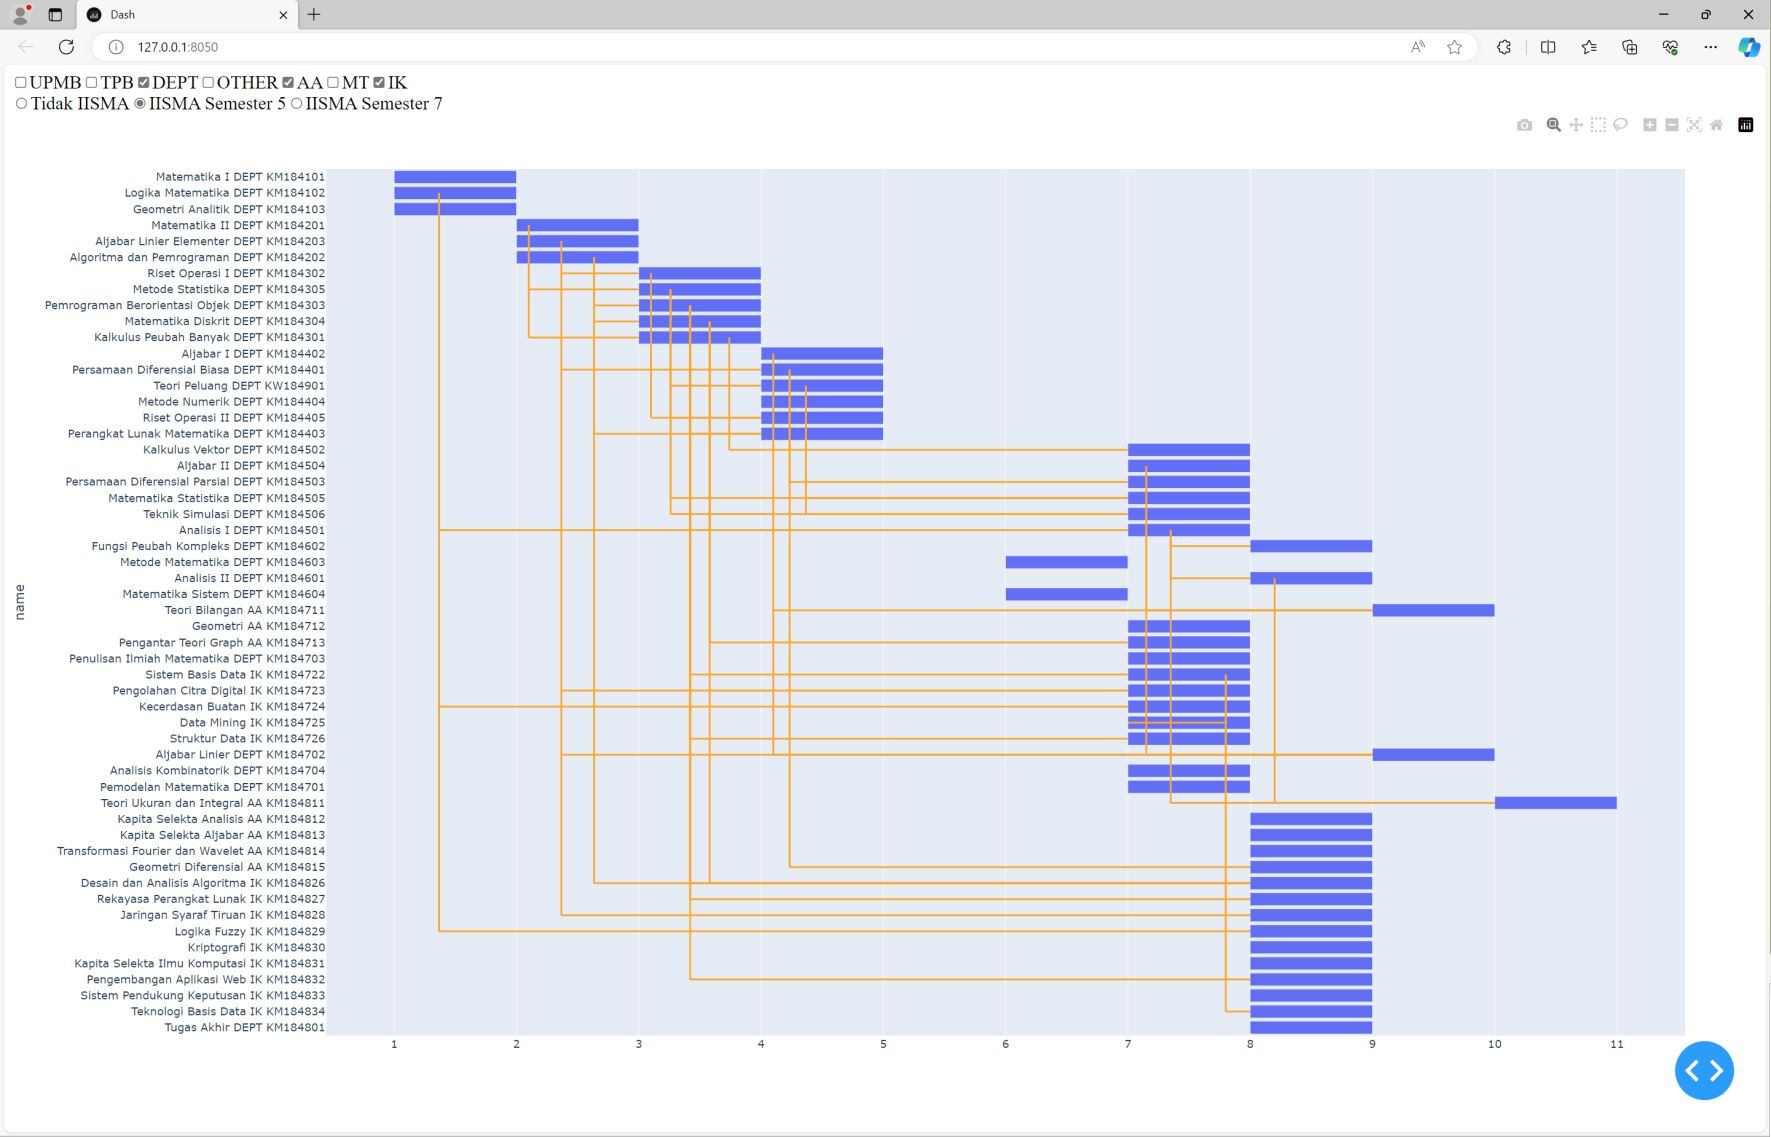
\includegraphics[height=3cm]{img/curriculum-graph}
\end{center}

This project was about analyzing my major curriculum program, and how events such as gap semesters or student exchange affects my study timeline. My modelling approach was to build a graph of prerequisite relationships between courses. Then, I am able to simulate how different scenarios in each semesters cascade into the following semesters.

\textit{(2021)} \textbf{Pseudo Image}

\textit{using C++, OpenGL, GLFW}

\begin{center}
	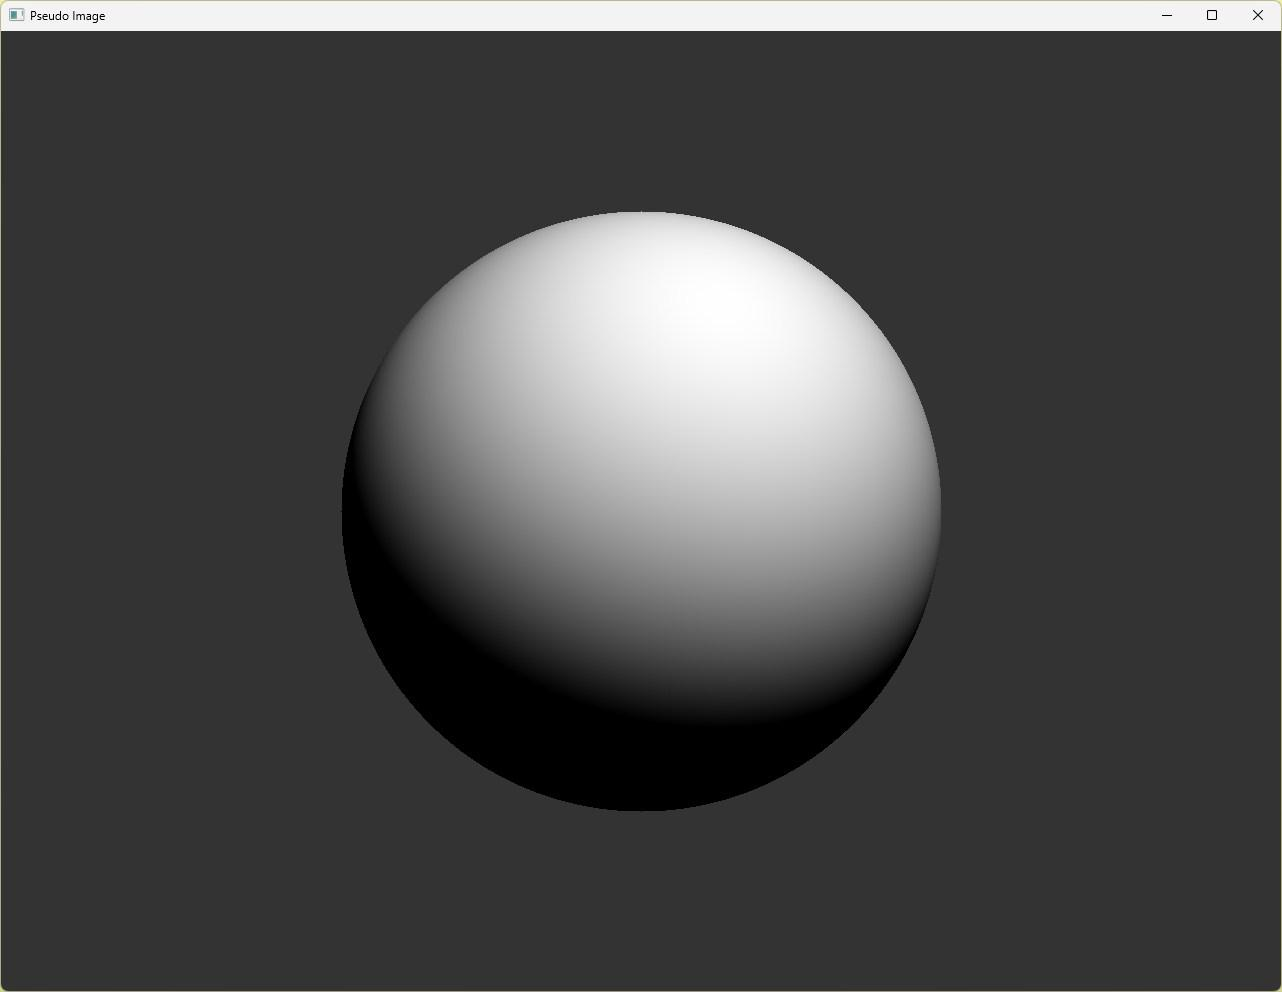
\includegraphics[height=3cm]{img/pseudo-image}
\end{center}

This project was my self taught effort at computer graphics. After successfully creating my first triangle using OpenGL, I set it up to cover the entire screen to create a blank canvas for shader experiments. Here, I created a ball using ray tracing logic in my shader.

\textit{(2021)} \textbf{Formal Boolean}

\textit{using C++}

\begin{center}
	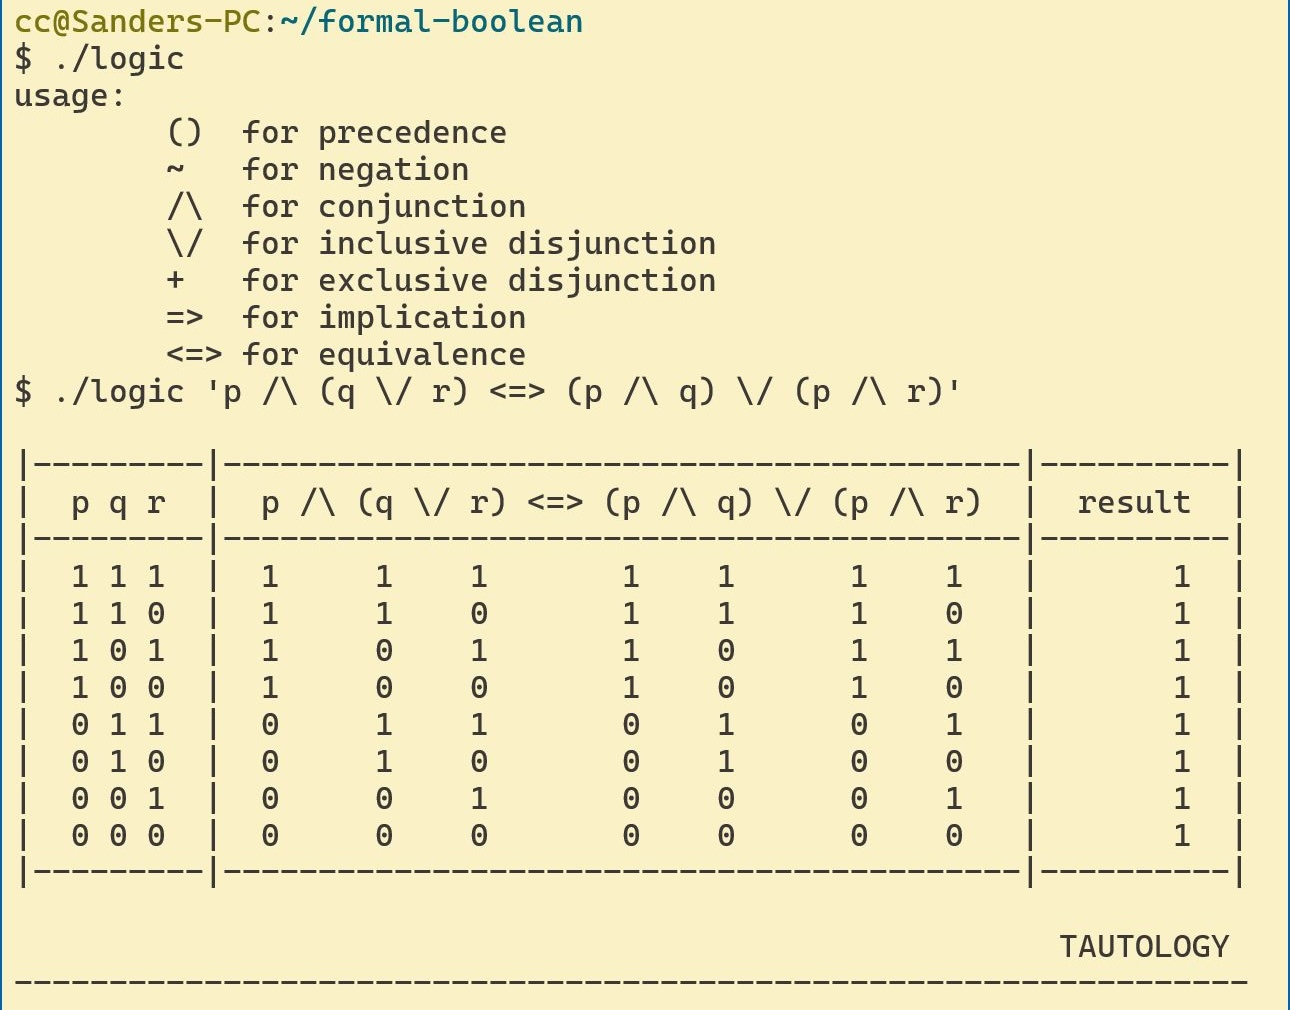
\includegraphics[height=3cm]{img/formal-boolean}
\end{center}

This project was built in my first year of university while studying mathematical logic. The program takes a Boolean expression as an input, and generates a truth table that lists all possible combinations of truth values for its variables. I wrote the parser from scratch without using external libraries.

\textit{(2020)} \textbf{Big Int}

\textit{using C++}

This project was my attempt at creating an arbitrary precision integer type. Here, I had to apply various classic mathematical concepts, such as algorithms for additions, subtractions, multiplications, and divisions. I also had to learn a lot about how to organize data structures in a library-like fashion.

\subsection{JavaScript experience}

My JavaScript experience came from my intensive use of it to create the Cobit Tools project mentioned above. Here, I used pure vanilla JavaScript without any libraries. I created utility functions that allows me to create DOMs declaratively, also taking advantage of my recently gained deep understanding of DOMs structure from the Refilter project. I also designed my UI to be immediate mode, where views are purely a function of state. Hence, I had to also work with JavaScript's standard event bus to implement the observer pattern, where I attach hooks that emits events, and creating a controller that listens for them.

\subsection{Node.js experience}

My experience with Node.js is more recent, about late 2025, where I started to get into Leetcode. I want to practice TypeScript, so I set up a devcontainer for it with Node.js inside. This also means that I have experience with the node:test framework, as this was what I used for offline testing of my exercises.

\subsection{C/Fortran experience}

I have a long history of experience using the C language from 2020 and back, before I had switched to C++. I used it mostly along together with OpenGL, creating visualizations for the Djikstra's algorithm.

\subsection{Interest in stdlib}

While Python and NumPy are the industry standards for numerical computing, they often feel like a "walled garden". It'd be great to have a standard equivalent in JavaScript.

With the advent of WebGPU, the browser is becoming a first-class platform for high-performance compute and scientific visualization. However, without a standardized, rigorous linear algebra suite comparable to NumPy, LAPACK, or BLAS, JavaScript developers are forced to "reinvent the wheel" or use fragmented, non-standard libraries.

I am drawn to stdlib because of its commitment to numerical rigor and its sophisticated architecture that treats multidimensional arrays and memory layout (row-major vs. column-major) with respect; that is, ndarray and BLAS/LAPACK parity.

\subsection{Version control}
Have you ever used Git for version control? Yes

\subsection{Contributions to stdlib}

\textit{PR \#11200:} feat: add iter/cartesian-square \\
Implemented the iter/cartesian-square resolving issue \#1334.

I created a complete package structure (lib/, test/, benchmark/, docs/) by analyzing existing patterns in array/cartesian-square and iter/counter. I demonstrated the ability to navigate the codebase, replicate the library's scaffolding, and following the coding standard.

\subsection{stdlib showcase}

WebGL Matrix Pipeline and 3D Visualization

Here, I hand-coded a WebGL rendering pipeline, and taking advantage of stdlib's linear algebra and array utilities.

\begin{itemize}
	\item I was also able to create frustum matrix as stdlib ndarray.

	\item @stdlib/blas/base/sgemm: Utilized for matrix multiplication to calculate Model-View-Projection (MVP) transformations.

	\item @stdlib/narray/flatten: Used to serialize ndarray structures into flat Float32Array buffers required for WebGL consumption.

	\item With stdlib, I also was able to convert between row-major memory layouts to the the column-major format required by WebGL.
\end{itemize}

\begin{center}
	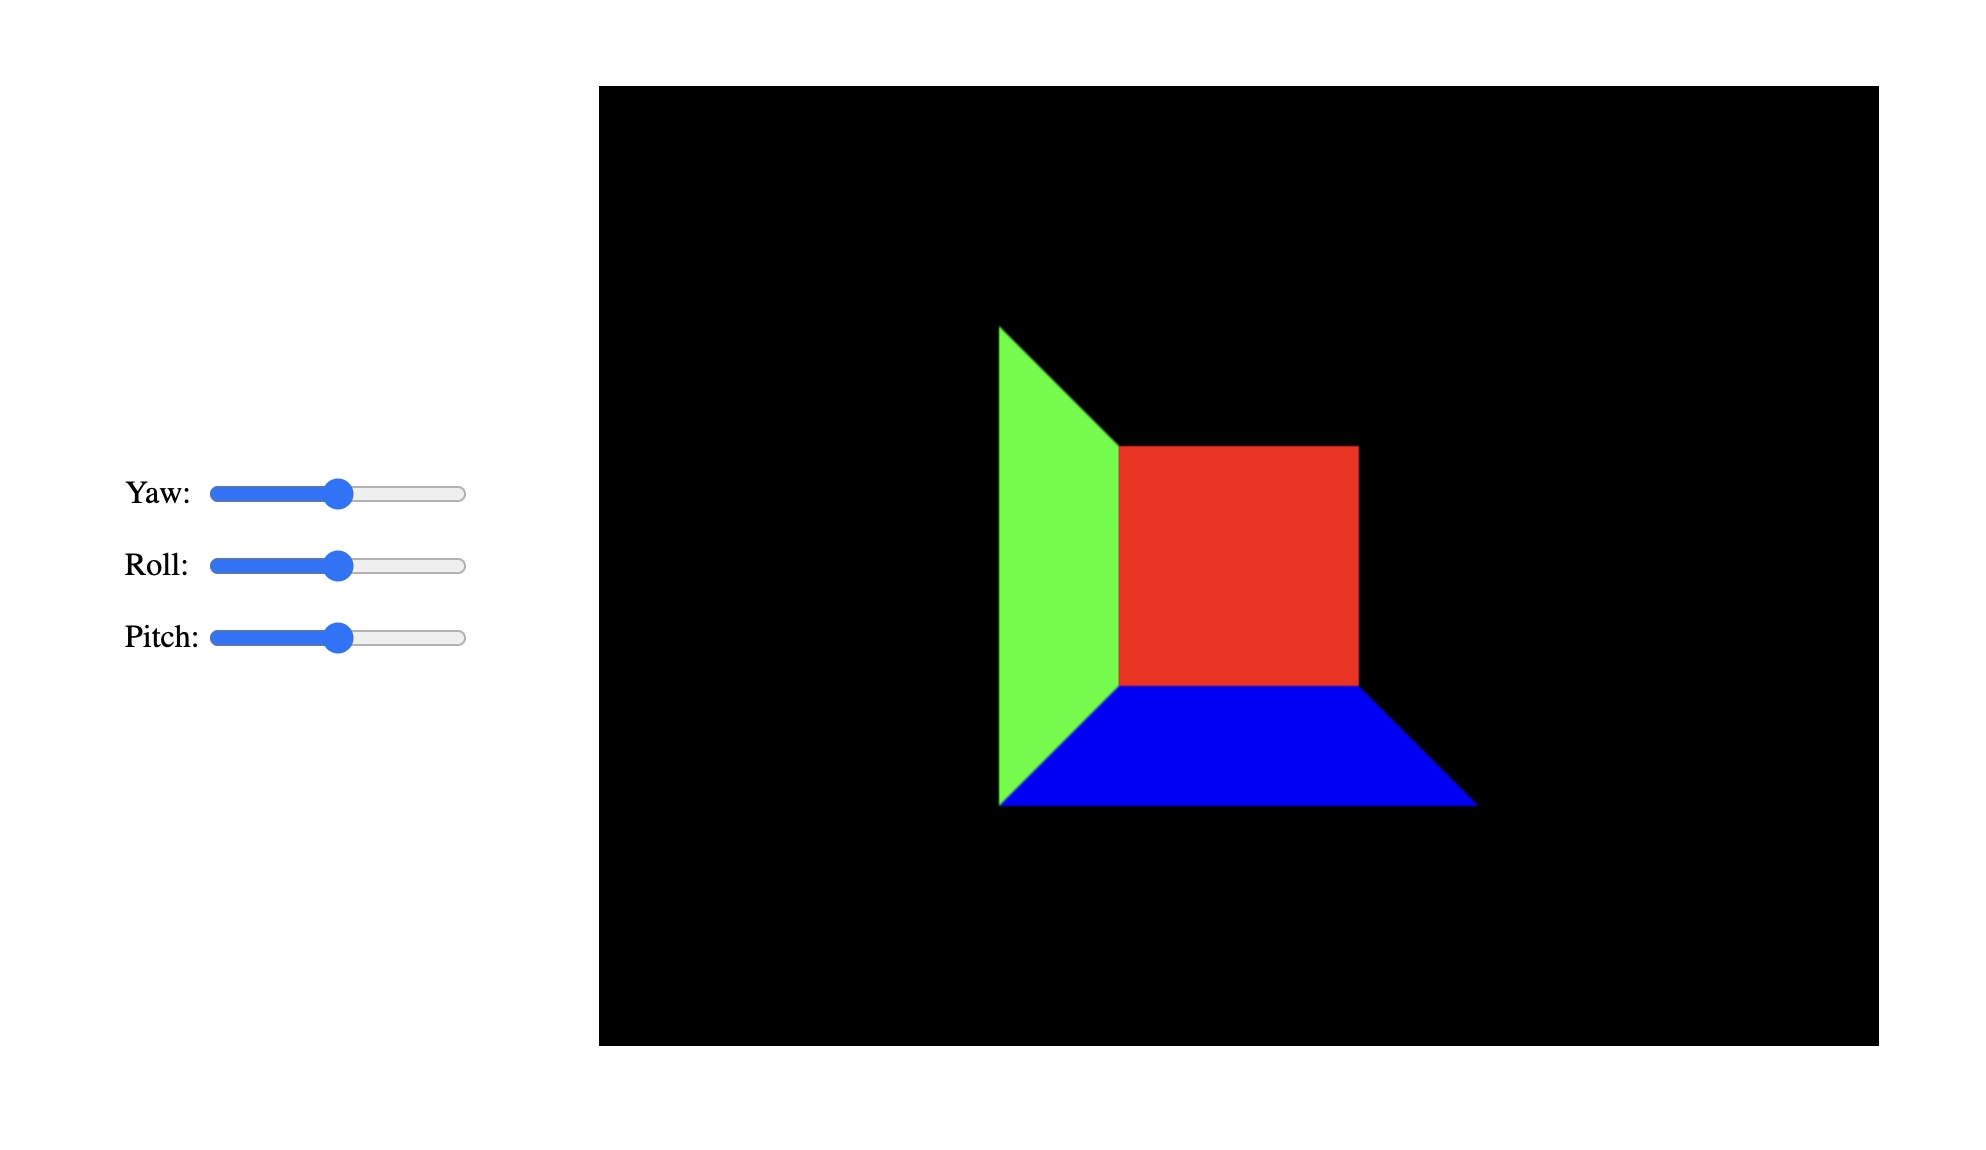
\includegraphics[height=4cm]{img/demo}
\end{center}

\textit{Demo link:} https://fikri-ajiwijaya.github.io/stdlib-demo/

\textit{stdlib-js use:} https://github.com/fikri-ajiwijaya/stdlib-demo/blob/dev/src/matrix.ts

\section{Project Description}

\subsection{Goals}

The primary goal of this project is to expand the linear algebra capabilities of stdlib-js by implementing core routines from the BLAS (Basic Linear Algebra Subprograms) and LAPACK specifications.

While stdlib already provides a robust ndarray foundation, many higher-level matrix operations required for scientific computing and computer graphics are currently missing or in early stages. My objective is to provide a "NumPy-equivalent" experience in JavaScript by delivering the following:

\begin{itemize}
	\item Expanded BLAS Support: Implementing missing Level 1 (vector-vector), Level 2 (matrix-vector), and Level 3 (matrix-matrix) routines to handle diverse memory layouts (row-major and column-major).

	\item Implementing fundamental algorithms such as LU Decomposition (with pivoting), QR Decomposition, and Cholesky Decomposition. These are the fundamental building blocks required for solving linear systems (\(Ax = b\)) and performing high-level matrix operations..

	\item Providing user-friendly functions for matrix inversion, determinants, and solving linear equations directly on stdlib ndarrays.

	\item For every routine, I will provide tests and complete JSDoc/TypeScript documentation.
\end{itemize}

\subsection{Why this project?}

As a recent Pure Mathematics graduate, I have spent years studying the abstract beauty of linear algebra.

What excites me most about this project is the timing. With the advent of WebGPU, the browser is finally capable of massive parallel computation. By contributing to stdlib, I am helping ensure that the CPU-side facilities do not lag behind while other parts of the web platform advance. The goal is to provide the necessary mathematical infrastructure so the JavaScript ecosystem can catch up to these hardware advancements.

I am particularly excited to work with the stdlib community because of their commitment to rigor and architecture. I want to apply my mathematical intuition to a codebase that values that level of precision.

\subsection{Qualifications}

My qualifications to execute this proposal are built on a dual foundation of theoretical mathematics and low-level systems programming.

\begin{itemize}
	\item I recently graduated with a Bachelor's degree in Pure Mathematics. My academic background has provided me with a deep understanding of linear algebra, including the numerical stability of algorithms, matrix decompositions, and vector space theory. My final project in Graph Theory required extensive use of NumPy for matrix algebra.

	\item My history with C (from before 2021), C++ and OpenGL has given me a strong grasp of memory management and the importance of data layout. Understanding the difference between row-major and column-major storage is not just a theoretical; it was a practical necessity in my WebGL and Pseudo Image projects to ensure CPU-to-GPU data parity.

	\item Through PR \#11200, I have already demonstrated that I can navigate the code base of stdlib. I am capable of implementing not just the core logic, but also the required JSDoc, TypeScript declarations, and benchmark suites that the organization demands.

	\item Projects like \textbf{Big Int} (implementing arbitrary-precision arithmetic from scratch in C++) and \textbf{Inkindo Billing} (multivariable linear regression) prove that I am comfortable implementing and testing numerical algorithms where precision is the primary requirement.
\end{itemize}

\subsection{Prior art}

The goal of bringing NumPy-like functionality to the JavaScript ecosystem has been approached by several existing libraries, each with different trade-offs.

\textbf{NumJs}

The most direct attempt at a "NumPy-like" experience. It provides an N-dimensional array object and basic linear algebra. However, it lacks the deep integration with low-level BLAS/LAPACK specifications that stdlib aims for, often prioritizing ease of use over strict numerical parity with Fortran/C reference implementations.

\textbf{TensorFlow.js}

Highly performant for machine learning via WebGL/WebGPU acceleration. While its Tensors are analogous to ndarrays, its API is specialized for computational graphs and gradient descent. For general-purpose scientific computing and pure linear algebra (like LU/QR decompositions on the CPU), it can be overly heavy and abstract.

\textbf{numpy-ts}

A modern, TypeScript-first implementation aiming for 100\% API compatibility. While its progress in implementing over 330 functions is impressive, stdlib distinguishes itself by its "scaffolded" approach—where every function is a standalone package with built-in benchmarks, documentation, and a focus on being a "standard library" rather than just a clone.

\textbf{jsnumpy}

A lightweight utility for basic array creation and simple 3D matrix manipulations. It serves as a proof of concept for basic matrix operations in JS but lacks the robustness required for production-level scientific computing.


\subsection{Commitment}

I am prepared to commit to this project as my primary professional focus for the duration of the Google Summer of Code.

I will dedicate 32 hours per week to development. My schedule is structured as 4 hours per day from Monday to Saturday, with a more intensive 8-hour session on Sunday. This consistent daily cadence, combined with a dedicated "deep work" day on Sundays, ensures that the project maintains steady momentum and allows for regular, incremental pull requests as per stdlib's architectural standards.

Over the 12-week coding period, this schedule totals 384 hours, which fully satisfies and exceeds the 350-hour requirement for a "Large" project.

\textit{(Community Bonding)} I am already active in the stdlib community through Zulip and GitHub (PR \#11200). I will continue to use the bonding period to audit current BLAS / LAPACK coverage and refine the implementation plan for the core solvers.

\textit{(Long-Term Commitment)} I view this project as the beginning of a long-term contribution to stdlib. I intend to be able to continue contributing towards stdlib after the 12-week period ends.

\pagebreak
\subsection{Schedule}

\textbf{Community Bonding Period}

Conduct an analysis to determine which prerequisite packages and functionality are currently missing to support high-level operations. Finalize the list of reference implementations in C and Fortran that will be used for parity testing.

\textbf{Week 1}

\textit{Goal:} BLAS for Triangular Matrices.

\textit{Deliverables:} PRs for routines such as trmv (triangular matrix-vector multiply) and trmm (triangular matrix-matrix multiply). These are essential for the "back-substitution" phase of the linear solvers.

\textbf{Week 2}

\textit{Goal:} BLAS for Symmetric/Hermitian Matrices.

\textit{Deliverables:} PRs for routines like symv (symmetric matrix-vector multiply) and syr (symmetric rank-1 update). These routines are the fundamental building blocks for the Cholesky decomposition.

\textbf{Week 3}

\textit{Goal:} High-level Matrix Multiplication API.

\textit{Deliverables:} Implement a user-friendly matmul or dot function that serves as the primary entry point for users, wrapping the low-level gemm and new Level 3 routines.

\textbf{Week 4}

\textit{Goal:} LU Decomposition.

\textit{Deliverables:} Implementation of LU decomposition with partial pivoting to ensure numerical stability for solving linear systems.

\textbf{Week 5}

\textit{Goal:} Matrix Inverse.

\textit{Deliverables:} Implement routines for calculating the matrix inverse based on the LU decomposition from Week 4.

\textbf{Week 6 (Midterm)}

\textit{Goal:} Cholesky Decomposition.

\textit{Deliverables:} Implementation of Cholesky decomposition for symmetric, positive-definite matrices. Midterm evaluation milestone.

\textbf{Week 7}

\textit{Goal:} QR Decomposition.

\textit{Deliverables:} Implementation of QR decomposition using Householder reflections, facilitating the solution of least-squares problems.

\pagebreak
\textbf{Week 8}

\textit{Goal:} Solving Linear Systems.

\textit{Deliverables:} Implement high-level solvers for \(Ax = b\) using previously implemented LU, QR, and Cholesky decompositions.

\textbf{Week 9}

\textit{Goal:} Eigenvalue Calculation (Part 1).

\textit{Deliverables:} Implement algorithms for calculating eigenvalues of symmetric matrices.

\textbf{Week 10}

\textit{Goal:} Singular Value Decomposition (SVD).

\textit{Deliverables:} Initial implementation of SVD routines for general matrices.

\textbf{Week 11}

\textit{Goal:} Code Freeze and Documentation.

\textit{Deliverables:} Finalize JSDoc, TypeScript declarations, and comprehensive unit tests for all implemented routines to match stdlib's rigorous standards.

\textbf{Week 12}

\textit{Goal:} Final Refinement and Benchmarking.

\textit{Deliverables:} Conduct performance benchmarking against reference implementations and address any remaining edge cases or mentor feedback.

\textbf{Final Week}

\textit{Goal:} Project Submission.

\textit{Deliverables:} Submission of the final project report and all merged/finalized code to the GSoC portal.

\subsection{Related issues}

This proposal is directly related to the following project idea issue in the stdlib-js Google Summer of Code repository:

\begin{itemize}
	\item {[RFC]}: Linear Algebra Functionality (Issue \#28): This issue outlines the goal of implementing core algorithms such as matrix multiplication, inverses, eigenvalue calculation, and SVD, as well as increasing the overall coverage of BLAS and LAPACK in stdlib.
\end{itemize}

\pagebreak
\section{Checklist}

\verb|- [x]| I have read and understood the Code of Conduct.

\verb|- [x]| I have read and understood the patch requirement which is necessary for my application to be considered for acceptance.

\verb|- [x]| I have read and understood the stdlib showcase requirement which is necessary for my application to be considered for acceptance.

\verb|- [x]| The issue name begins with [RFC]: and succinctly describes your proposal.

\verb|- [x]| I understand that, in order to apply to be a GSoC contributor, I must submit my final application to https://summerofcode.withgoogle.com/ before the submission deadline.

\end{document}
